
\documentclass{beamer}
\usepackage{beamerthemesplit}
\usepackage{graphics}
\usepackage{pstricks}
\usepackage[T2A]{fontenc}			% кодировка
\usepackage[utf8]{inputenc}			% кодировка исходного текста
\usepackage[english,russian]{babel}	% локализация и переносы
%grek
\usepackage{ tipa }
\usepackage{ amssymb }

\usepackage{caption, subcaption}
\usepackage{wasysym}
\usepackage{textcomp}
\usepackage{pgf}  



\setbeamercovered{dynamic} % overlays not yet revealed will faintly appear
\usepackage{indentfirst}


\graphicspath{ {img/} }

\title{Научная Мастерская}
\author{Михаил Соловьянов}


\begin{document}

\frame{
   \begin{center}
    \huge{Введение в цифровую электронику\\ создание цифрового сумматора}\\
    \vspace{48pt}
    \Large{Соловьянов Михаил}\\
    \vspace{18pt}
    \large{\today}
  \end{center}
}




\frame{\frametitle{Используемые элеметы (на человека)}
  \begin{center}
  \LARGE
	\begin{enumerate}
	\item  Макетная плата - 1шт.
	\item Плата питания -1 шт.
	\item Провод питания USB - 1шт.
	\item Светодиоды - 4 шт.
	\item Резисторы - 4шт.
	\item Микросхемы : лоигческие вентили 2 шт.
	\item Провода
	\end{enumerate}
  \end{center}
}





\frame{
  \begin{center}
    \includegraphics[width=\textwidth]{dig.png}
  \end{center}
}




\frame{\frametitle{Процессор intel 4004}
  \begin{center}
    \includegraphics[width=\textwidth]{1.jpg}
  \end{center}
}


\frame{
  \begin{center}
    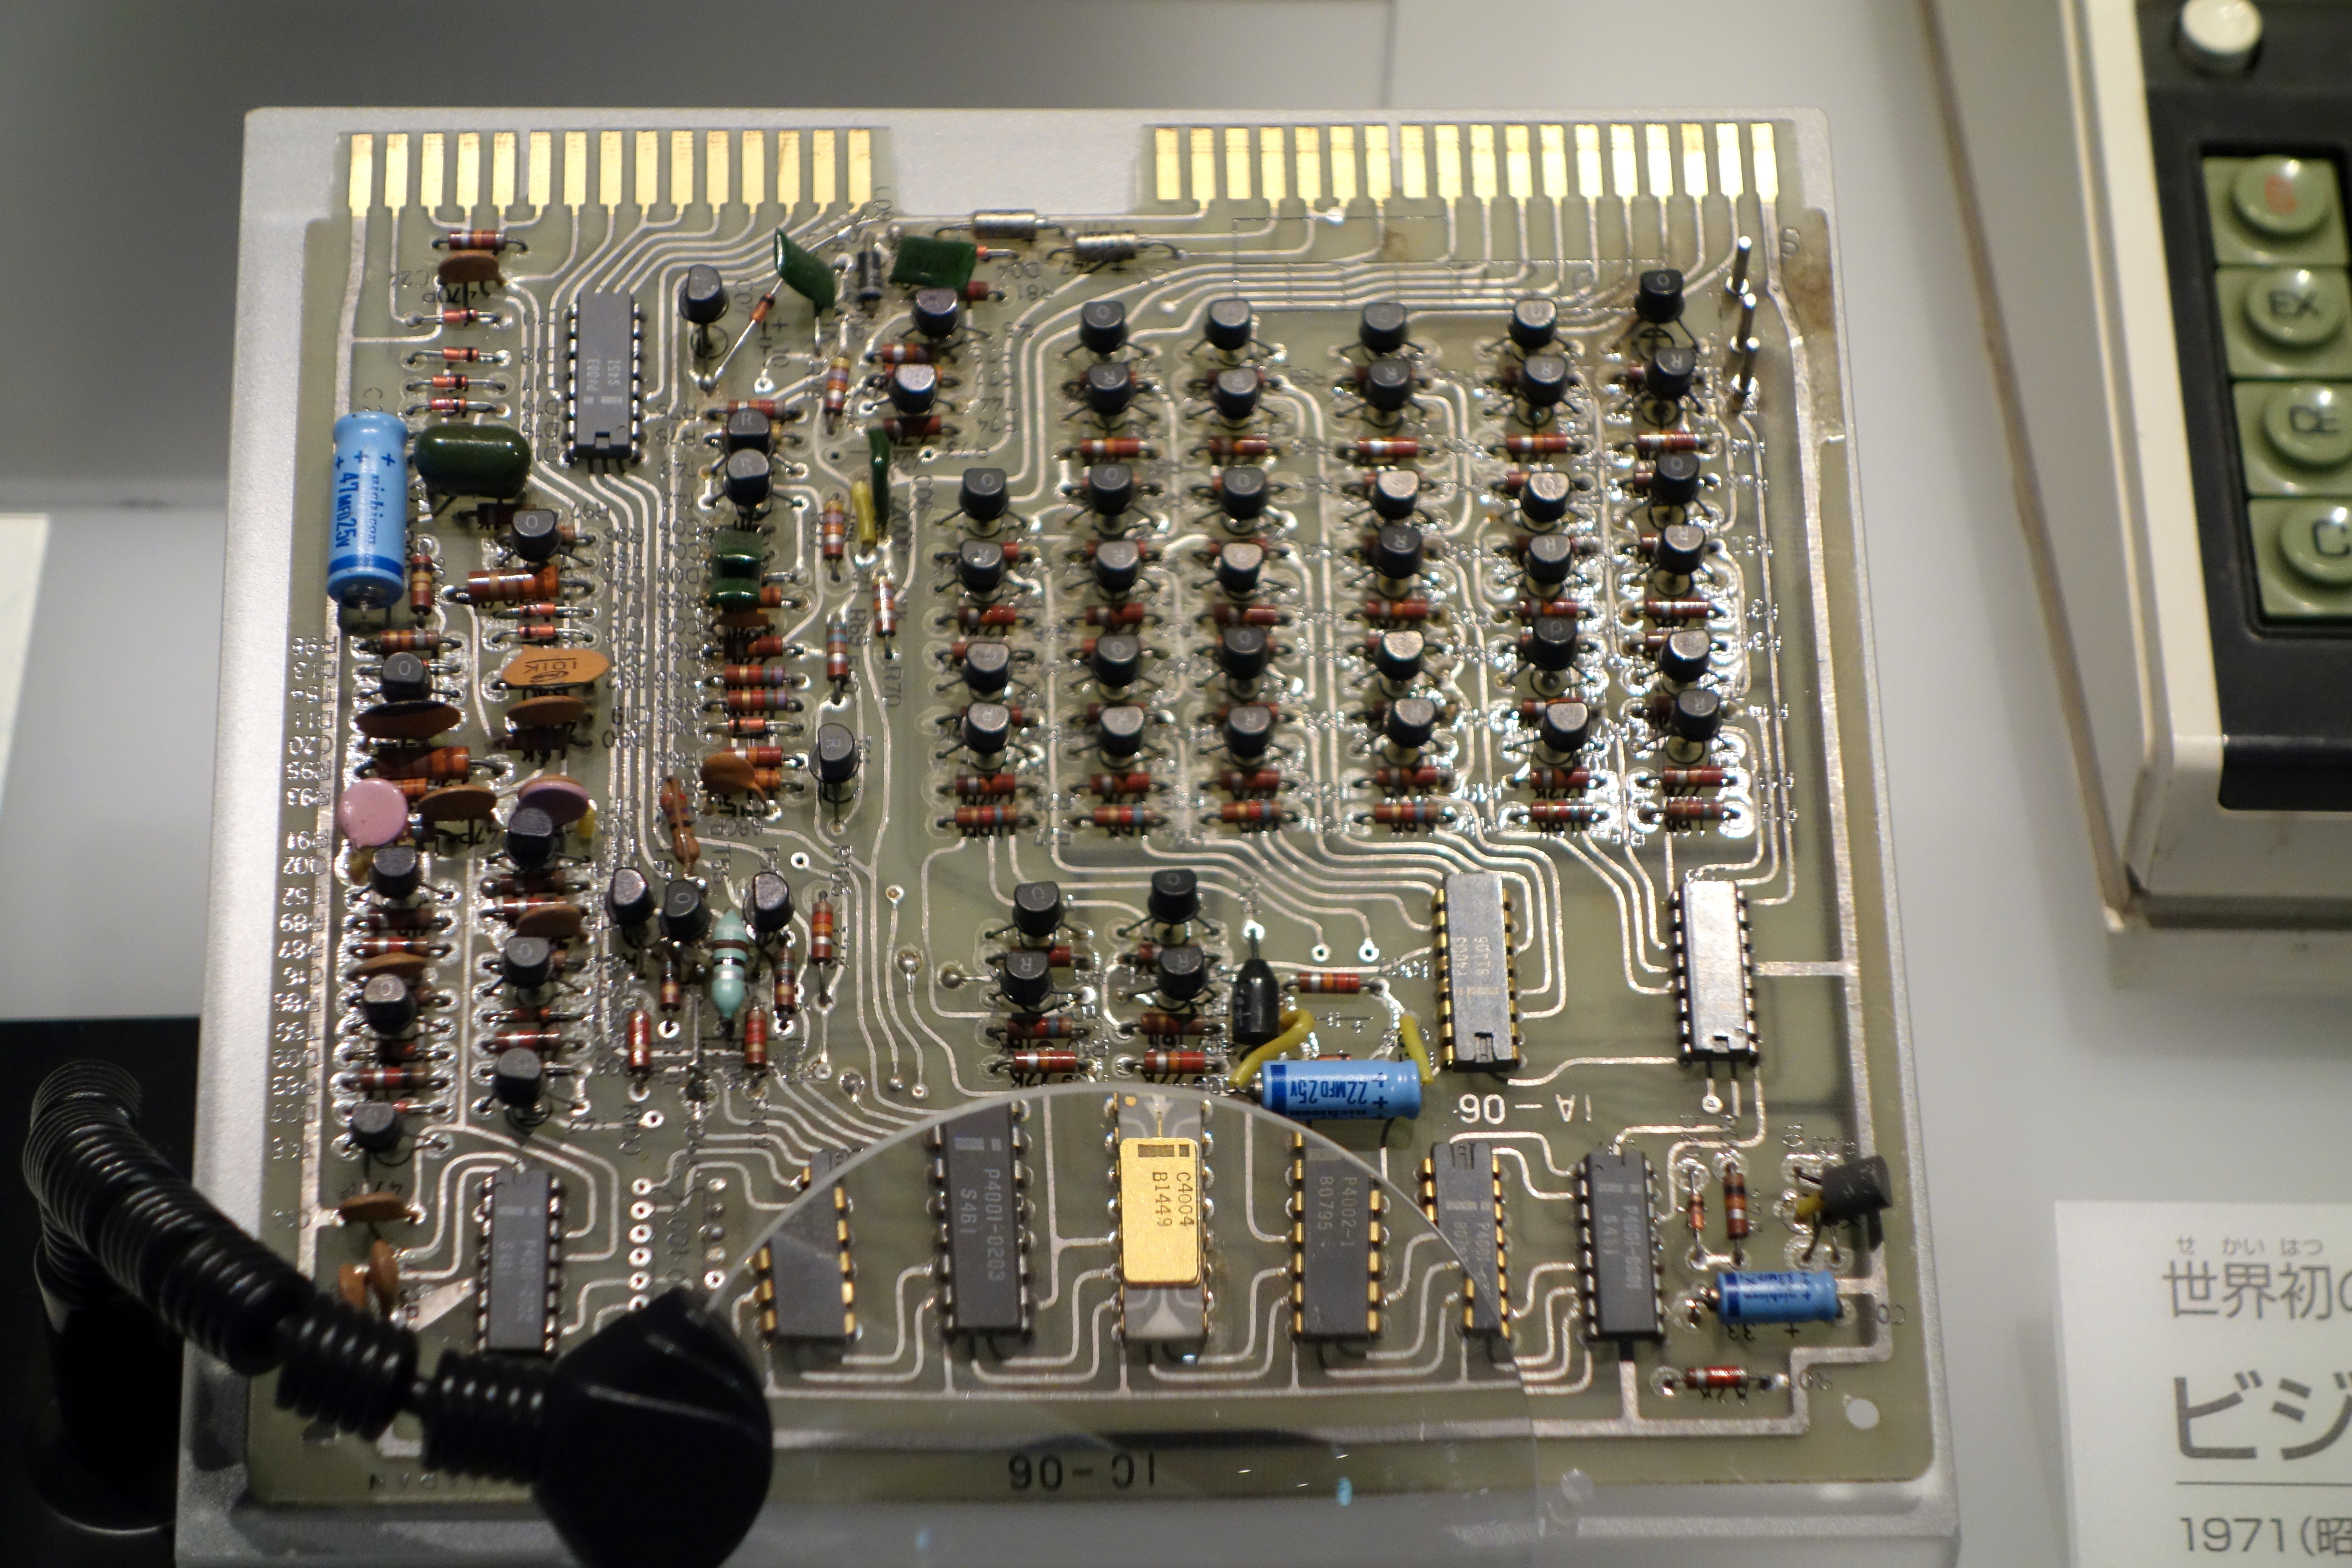
\includegraphics[width=\textwidth]{2.jpg}
  \end{center}
}


\frame{\frametitle{Инструкция процессора}
  \begin{center}
    \includegraphics[width=\textwidth]{calc.png}
  \end{center}
}

\frame{
  \begin{center}
    \includegraphics[width=1.05\textwidth]{assembler.png}
  \end{center}
}



\frame{

  \begin{center}
  \large {Цифровая электроника:}
	\begin{enumerate}
	 \item Электричество
      \item   Математика  -- двоичная
      \item  Логика -- Алгебра логики
      \item  Электроника
	\end{enumerate}
  \end{center}
}





%------------------------------------ELEC!!!----------------------------------
\frame{\frametitle{Что такое электрон?}
  \begin{center}
 \includegraphics[width=0.95\textwidth]{Electron-Shell.png}
  \end{center}   }


\frame{

  \begin{center}
  \huge
  Если точнее, но не очень наглядно:
  $$ i\hbar \frac{\partial }{\partial t } | \psi (t) \rangle =  \hat{H} \psi (t) \rangle$$
  \end{center}   }

\frame{
  \begin{center}
   \LARGE{Электрический ток -- упорядоченное движение заряженных частиц}
  \end{center}
}




\frame{
  \begin{center}
  \huge
  Будем представлять их так:
 \includegraphics[width=0.95\textwidth]{crowd.jpg}
  \end{center}   }





\frame{
  \begin{center}
 \includegraphics[width=0.95\textwidth]{elec.png}
  \end{center}   }






\frame{
  \begin{center}
 \includegraphics[width=0.95\textwidth]{battery.png}
  \end{center}   }


\frame{
  \begin{center}
   \includegraphics[width=0.8\textwidth]{c1.png}\\
   \LARGE{ $$ I = \frac{U}{R} $$}
   
  \end{center}
}


\frame{
  \begin{center}
   \includegraphics[width=0.6\textwidth]{c1.png}\\
  \includegraphics[width=0.6\textwidth]{c2.png}\\
   
  \end{center}
}




\frame{
  \begin{center}
 \includegraphics[width=0.95\textwidth]{pic-Diode.png}
  \end{center}   }





% WORK BY HANDS



%PCB
\frame{
  \begin{center}
    \includegraphics[width=0.95\textwidth]{maket_1.png}\\
  \end{center}
}

\frame{
  \begin{center}
    \includegraphics[width=0.95\textwidth]{maket_2.png}\\
  \end{center}
}



\frame{
  \begin{center}
    \includegraphics[width=0.3\textwidth]{diode_for_dummy.png}\\
  \end{center}
}

\frame{\frametitle{Как подключать диод!}
  \begin{center}
 \includegraphics[width=0.7\textwidth]{diode.png}\\
 \vspace{0.5cm}
  \includegraphics[width=0.7\textwidth]{diode1.png}\\
  \end{center}
}


\frame{
  \begin{center}
    \includegraphics[width=\textwidth]{on-off.png}
  \end{center}
}



% NOW BINARY

\frame{\frametitle{Двоичное исчисление?}
  \begin{center}
    \includegraphics[width=0.5\textwidth]{bin_mem.jpg}
  \end{center}
}



\frame{
  \begin{center}
    \includegraphics[width=0.5\textwidth]{pic-bin.png}
  \end{center}
}



\frame{
  \begin{center}
    \includegraphics[width=0.8\textwidth]{bin_led.png}
  \end{center}
}





\frame{
  \begin{center}
 \LARGE{Числа -- это то, что состоит из символов и то, чем мы описываем количество}
  \end{center}
}





\frame{
  \begin{center}
    \includegraphics[width=\textwidth]{bin_calc.png}
  \end{center}
}




\frame{\frametitle{Что такое транзистор?}
  \begin{center}
 \includegraphics[width=0.7\textwidth]{valve.png}
  \end{center}   }




\frame{

 \includegraphics[width=\textwidth]{pic-valve.png}

  }


\frame{
  \begin{center}
 \includegraphics[width=\textwidth]{circuit.png}
  \end{center}   }

\frame{
  \begin{center}
 \includegraphics[width=0.9\textwidth]{npmos.png}
  \end{center}   }


\frame{
  \begin{center}
    \includegraphics[width=0.8\textwidth]{transistor.jpg}\\
    Вот таких вот транзисторов было выпущено не меньше чем спичек!
  \end{center}   }

%------------------------------------------LOGIC!!!!!!!!----------------------------------------


\frame{\frametitle{GATE level? Алгебра логики?! Это же так просто!}
  \begin{center}
    \includegraphics[width=1.05\textwidth]{minecraft.jpg}
  \end{center}
}


\frame{
  \begin{center}
    \includegraphics[width=1.05\textwidth]{minecraft_redstone.png}
  \end{center}
}



\frame{
  \begin{center}
    \includegraphics[width=\textwidth]{elem.png}
  \end{center}
}








\frame{\frametitle{Операция "НЕ"}
  \begin{center}
  \LARGE{
    \begin{table}[]
\begin{tabular}{|l|l|l|}
\hline
\multicolumn{2}{|l|}{\includegraphics[width=8cm]{not.png}} \\ \hline
$A$ &$ \overline{A}$ \\ \hline
1 & 0  \\ \hline
0 & 1 \\ \hline

\end{tabular}
\end{table}}
  \end{center}
}


\frame{\frametitle{Инвертор}
  \begin{center}
    \includegraphics[width=0.7\textwidth]{inv.png}\\

  \end{center}   }


\frame{
  \begin{center}
    \includegraphics[width=0.7\textwidth]{inv1.png}\\

  \end{center}   }





\frame{
  \begin{center}
    \includegraphics[width=0.7\textwidth]{inv2.png}\\

  \end{center}   }



\frame{
  \begin{center}
    \includegraphics[width=0.7\textwidth]{inv3.png}\\

  \end{center}   }
























\frame{\frametitle{Операция "ИЛИ"}
  \begin{center}
  \LARGE{
    \begin{table}[]
\begin{tabular}{|l|l|l|}
\hline
\multicolumn{3}{|l|}{\includegraphics[width=6.5cm]{or.png}} \\ \hline
$A$ &$ B$ & $A+B $\\ \hline
1 & 0 & 1 \\ \hline
0 & 1 & 1 \\ \hline
0 & 0 & 0 \\ \hline
1 & 1 & 1 \\ \hline
\end{tabular}
\end{table}}
  \end{center}
}


\frame{

  \begin{center}
  \LARGE{Тебе купили в парке мороженое \textbf{или} лимонад ,да?}
  \end{center}
}



\frame{\frametitle{Операция "И"}
  \begin{center}
  \LARGE{
    \begin{table}[]
\begin{tabular}{|l|l|l|}
\hline
\multicolumn{3}{|l|}{\includegraphics[width=8cm]{and_true.png}} \\ \hline
$A$ &$ B$ & $A \times B $\\ \hline
1 & 0 & 0  \\ \hline
0 & 1 & 0 \\ \hline
0 & 0 & 0 \\ \hline
1 & 1 & 1 \\ \hline
\end{tabular}
\end{table}}
  \end{center}
}




\frame{
  \begin{center}
  \LARGE{
    Тебе купили в парке мороженое  \textbf{и} лимонад ,да?}
  \end{center}
}


%%%%%%


\frame{
  \begin{center}
    \includegraphics[width=0.8\textwidth]{door.png}
  \end{center}
}


\frame{
  \begin{center}
    \includegraphics[width=0.8\textwidth]{door2.png}
  \end{center}
}






\frame{\frametitle{Операция "ИСКЛЮЧАЮЩЕЕ ИЛИ"}
  \begin{center}
  \LARGE{
    \begin{table}[]
\begin{tabular}{|l|l|l|}
\hline
\multicolumn{3}{|l|}{\includegraphics[width=8cm]{or_true.png}} \\ \hline
$A$ &$ B$ & $A\oplus B $\\ \hline
1 & 0 & 1 \\ \hline
0 & 1 & 1 \\ \hline
0 & 0 & 0 \\ \hline
1 & 1 & 0 \\ \hline
\end{tabular} 
\end{table}}
  \end{center}
}



\frame{
  \begin{center}
  \LARGE{Рассмотрим как такой элемент выглядит в реальности}
  \end{center}
}


\frame{\frametitle{Микросхемы!}
  \begin{center}
 \includegraphics[width=0.85\textwidth]{DIP14.png}\\
 \large{Корпус DIP14}
  \end{center}
}



\frame{
  \begin{center}
 \includegraphics[width=0.7\textwidth]{XOR.PNG}\\
 \large{Корпус DIP14}
  \end{center}
}

\frame{
  \begin{center}
  \LARGE{Для чего он нам нужен? Для сложения!}
  \end{center}
}


%---------------------------------LOGIC







\frame{
  \begin{center}
   \includegraphics[width=1.1\textwidth]{1+0.png}\\
  \end{center}
}



\frame{
  \begin{center}
   
\includegraphics[width=0.8\textwidth]{sum.png}\\
  \end{center}
}


\frame{
  \begin{center}
   \includegraphics[width=\textwidth]{h_adder.png}\\
  \end{center}
}










%------------------------------------------PRAC!!!!!!!!----------------------------------------













\frame{
  \begin{center}
 \LARGE{Вопросы?}
  \end{center}
}


\frame{
  \begin{center}
  \LARGE{За работу!}
    \includegraphics[width=0.95\textwidth]{index.jpg}\\
  \end{center}
}


\frame{
  \begin{center}
    \includegraphics[width=\textwidth]{project.png}\\
    \large{Итоговая схема}
  \end{center}
}



\frame{\frametitle{Итоги}

  \begin{center}
  \large {Мы узнали:}
	\begin{enumerate}
      \item   Из чего состоит компьютер
      \item  Что такое двоичное счисление 
      \item  Как складывать числа с помощью простых логических элементов
	\end{enumerate}
  \end{center}
}





\frame{\frametitle{Отличие от курса}

  \begin{center}
  \large {Данный мастер класс не отражает темп освоения курса, но отражает общий подход и фундаментальность  конечного материала научной мастерской. В частности в курсе предусмотрены:}
	\begin{enumerate}
      \item Работа дома и консультация с наставником через социальные сети.
      \item Более постепенное освоение материала.
      \item  Творческие проекты для каждого отдельного ученика вне сжатых сроков.
	\end{enumerate}
  \end{center}
}





\frame{
  \begin{center}
\LARGE{Причины возникновения направления}
  \end{center}
}


\frame{ 
  \begin{center}
  Спасибо за внимание! \smiley{}\\
  \vspace{2cm}
    {\Huge \red The end}
  \end{center}
}



%-------------------------------- UNDER DOG------------------------------------------
\frame{\frametitle{Вентиль - "И"}
  \begin{center}
    \includegraphics[width=0.6\textwidth]{nand.png}\\

  \end{center}   }
  
  \frame{\frametitle{Вентиль "ИЛИ"}
  \begin{center}
    \includegraphics[width=0.4\textwidth]{or_gate.png}\\

  \end{center}   }




\frame{\frametitle{Топология ячейки памяти}
\begin{center} 
 \includegraphics[width=0.4\textwidth]{cell_h.png}
 \includegraphics[width=0.4\textwidth]{FRAM-fig1.png}
\end{center}
}





\frame{\frametitle{Конструкция усовершенствованного дифференциального неразрушающего  усилителя чтения }
 \begin{center} 

       \begin{tabular}{cl}  
         \begin{tabular}{c}
            \includegraphics[width=0.5\textwidth]{SA.png}
           \end{tabular}
           & \begin{tabular}{l}
             \parbox{0.4\linewidth}{%  change the parbox width as appropiate
             \includegraphics[width=0.4\textwidth]{AMP_v.png}
    }
         \end{tabular}  \\
\end{tabular}
 \end{center}
}




\end{document}